% !TEX root = ../main_orange.tex


Particle physics is an area of physics that deals with the behaviour of the most basic constituents of matter and their mutual interaction. This section wants to serve as a \textbf{very} compact summary of the main aspects of particle physics that you need to know to be able to run this experiment. The book which is used in the particle physics module here at the University of Sussex is the one listed in Ref.~\cite{shaw}: you may want to have a look there for more details. 

Particles are very small, and, for what concern this experiment, very fast as well. A mathematically sound physical theory of particle physics needs to be compliant with the laws of quantum mechanics and (special) relativity. The standard formulation of particle physics is done in terms of a Quantum Field Theory. We will avoid almost any reference to QFT: this will imply that in some places you will have to ``believe'' some of the results that will be presented. 

Depending of the property one is interested in, particles can be grouped in a few different ways:

\begin{itemize}
\item If one is interested in their spin properties, particles are divided into \textbf{fermions}, whose spin is fractional (like $1/2$, $3/2$, etc.), and \textbf{bosons}, whose spin is integer. All elementary particles that constitute ordinary matter (the up and down quarks, the electrons) are fermions. All particles that mediate an interaction (the photon, the Higgs boson, etc.) are bosons.
\item If one is interested in their spacial size, particles are divided into \textbf{elementary} (more on them later), that should be imagined essentially as a geometrical point in space, with no physical size, and \textbf{composite}, that is, bound states of other particles. Examples of elementary particles are the electron and the quarks. Composite particle examples are the proton and the neutron. 
\item If one is interested in the interactions they feel, particles are divided into \textbf{leptons}, that interact through gravity and the electroweak force, and \textbf{hadrons} which interact through gravity, the electroweak force and the strong nuclear force. The electron and neutrinos are leptons, the quarks are hadrons.
\end{itemize}

Other groupings are possible: we will introduce them if and when they will be needed. In the following, the word ``particle'' will be used with the meaning of ``elementary particle'', unless stated otherwise.

Particles are objects with a mass of the order of that of the proton. There are large variations on this order of magnitude: the heaviest known elementary particle is the top quark, whose mass is about 172 times that of the proton. The electron is the lightest massive particle, with a mass of about half of a thousandth of a proton. Massless particles exist as well (the photon mass is zero, that of the neutrinos is very small although not zero).

\begin{figure}[tb] 
	\centering
	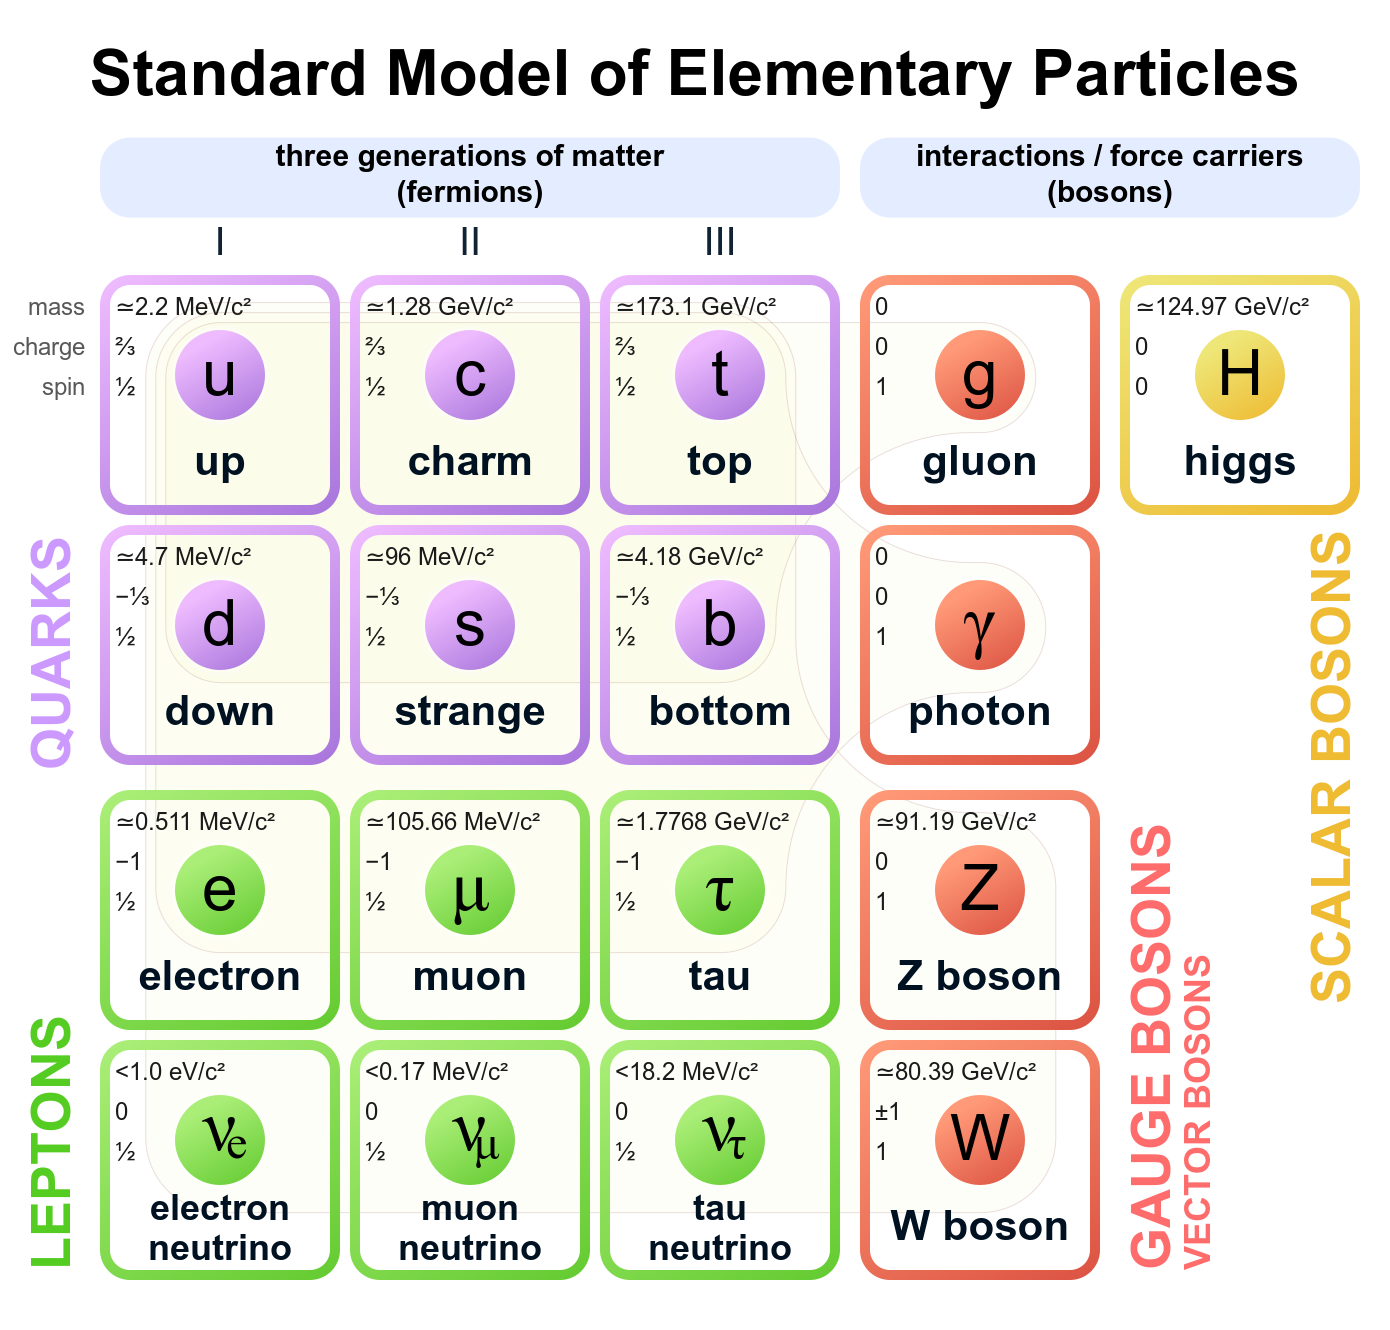
\includegraphics[width=0.5\columnwidth]{Figures/Standard_Model_of_Elementary_Particles.png}
	\caption{Particle content of the Standard Model of Particle Physics. For each particle, the mass, the charge and the spin are reported. Please bear in mind that the mass of light quarks ($u$, $d$, $s$) is not straightforward to define and estimate, given that no free quark can be observed. Taken from Ref.~\cite{SM_wikipedia}.}
		\label{tab:SM}	
\end{figure}


\section{The Standard Model of Particle Physics} 

The best theory of particle physics we have available is the so--called Standard Model of Particle Physics (SM in the following). It specifies the full list of particles, their properties and their interactions. Table~\ref{tab:SM} summarises the particle content of the SM. There are three leptonic families (in green). In each leptonic family, there is a charged lepton and a neutrino of the same flavour. There are also three quark families (in purple). In each quark family there is a quark with charge $+\frac{2}{3}$ and one with charge $-\frac{1}{3}$. Each quark defines its own flavour. Not shown in the table: for each particle family there is an identical family composed by anti-particles. So, for the family composed by the electron and its neutrino, there is a family composed by a positively charged electron (the positron) and an antineutrino, and same for the quarks. 

There are also bosons, that mediate the interactions between the particles in the leptonic and quark families (in red). These are: 
\begin{itemize}
\item The photon, that mediates the electromagnetic interaction between charged particles. 
\item The $W^+, W^{-}$ and $Z$ bosons, which mediate the weak interaction between leptons and between quarks. 
\item The gluons, that mediate the strong nuclear interaction between quarks. 
\end{itemize} 

Finally, the Higgs boson is shown in yellow: it interacts with all particles with an intensity that is proportional to the particle mass. 

We will use a helpful graphical tool to represent interactions between particles. These are the Feynman diagrams. Please bear in mind that we will use them only as a graphical tool, but they are actually a representation of quantitative mathematical expressions that allow to precisely calculate how likely a given process is to occur. In these graphs, we will always represent incoming particles on the left and outgoing particles on the right. 

There are important rules that have to be respected when drawing possible Feynman diagrams:
\begin{enumerate}
\item Electric charge, momentum, energy and angular momentum are always conserved at a vertex.
\item Fermions are represented with arrows. An incoming (in a vertex) fermion is represented with an incoming arrow, while an outgoing fermion is represented with an outgoing arrow. For anti-fermions, rules are reversed: an incoming anti-fermion is represented with an outgoing arrow, while an outgoing anti-fermion is represented with an incoming arrow. See examples in Figure~\ref{fig:feyn_example}. 
\item The total number of leptons has to be conserved. Each lepton contributes to the number of leptons with an additive $+1$, while each anti-lepton with an additive $-1$.
\item Likewise, the total number of quarks has to be conserved. Each quark contributes with an additive $+\frac{1}{3}$, while each anti-quark with an additive $-\frac{1}{3}$.
\item As a consequence of rule 1 for angular momentum, a three-line vertex can only be: two fermions and a boson; three bosons.
\item Gluons interact only with quarks and other gluons. 
\item The $Z$ and $\gamma$ bosons always conserve the flavour. So, $Ze^+e^-$, $Zu\bar{u}$, $\gamma c\bar{c}$ are perfectly legal vertices, $Z e^+ \mu^{-}$, $Zc\bar{s}$ and $\gamma e^-\mu^+$ are not.
\item The $Z$ boson does not interact with the photon.
\item The $W$ boson interaction conserves the leptonic flavour. So $We\bar{\nu}_e$ is a legal vertex, but $We\bar{\nu}_{\mu}$ is not. 
\end{enumerate}

Figure~\ref{fig:feyn_example}~\footnote{In this handbook, we will always deal with so-called \textit{leading-order} Feynman diagrams. If you want to know more about \textit{higher order} Feynman diagrams, please consult Ref.~\cite{shaw}. We will also neglect possible leading order Feynman diagram vertices that include more than three lines.} shows examples of allowed Feynman diagrams, while Figure~\ref{fig:forbidden_feyn} shows some processes which are not allowed. 

 \begin{figure}[!h]
\begin{center}
\subfigure[Production of a Z boson decaying into a $\mu\bar{\mu}$ pair at an electron-positron collider.]{
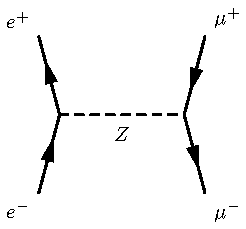
\includegraphics[width=0.2\textwidth]{./Figures/ee_to_Zmumu.eps}
}
\hfill
\subfigure[A diagram for $W$ production at a hadron collider, followed by the $W$ decay into two quarks.]{
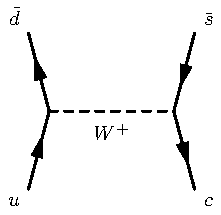
\includegraphics[width=0.2\textwidth]{./Figures/ud_to_Wcs.eps}
}
\hfill
\subfigure[A diagram for $t\bar{t}$ production at a hadron collider.]{
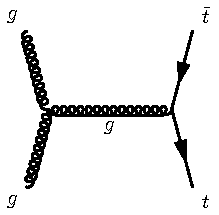
\includegraphics[width=0.2\textwidth]{./Figures/gg_to_ttbar.eps}
}
\hfill
\subfigure[Higgs boson production via the so-called gluon fusion process, followed by $H\rightarrow\gamma\gamma$, at a hadron collider. Both the gluons and the photons are massless particles, the Higgs boson couples to them through intermediate particles.]{
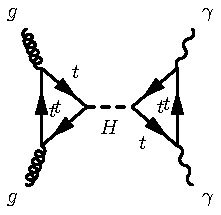
\includegraphics[width=0.2\textwidth]{./Figures/Higgs_gluonFusion.eps}
}
\end{center}
\caption{Examples of valid Feynman diagrams. For each of them, the fermion lines do not stop within the diagram, rather they enter and exit the diagram fully. This is a consequence of angular momentum and charge conservation.}
\label{fig:feyn_example}
\end{figure}

 \begin{figure}[!h]
\begin{center}
\subfigure[Violation of charge conservation at the $W$ production vertex.]{
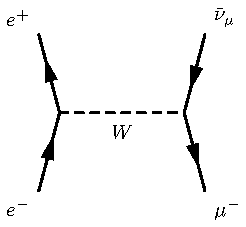
\includegraphics[width=0.2\textwidth]{./Figures/ee_to_Wmumu.eps}
}
\hfill
\subfigure[Flavour violation at the $Z$ decay vertex. The $Z$ boson only couples to leptons and quarks of the same flavour.]{
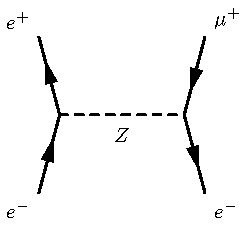
\includegraphics[width=0.2\textwidth]{./Figures/ee_to_Zemu.eps}
}
\hfill
\subfigure[Charge conservation violation at the Higgs boson production vertex.]{
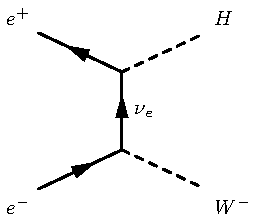
\includegraphics[width=0.2\textwidth]{./Figures/ee_to_WH.eps}
}
\hfill
\subfigure[Four-fermion interaction vertices do not exist in the Standard Model.]{
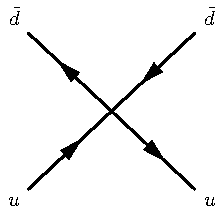
\includegraphics[width=0.2\textwidth]{./Figures/ud_to_ud.eps}
}
\hfill
\subfigure[There is a broken fermion line at both vertices (violation of charge, angular momentum, baryon number conservation).]{
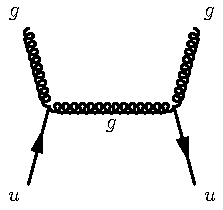
\includegraphics[width=0.2\textwidth]{./Figures/ug_to_g.eps}
}
\hspace{1cm}
\subfigure[The Higgs boson does not couple directly with particles with no mass.]{
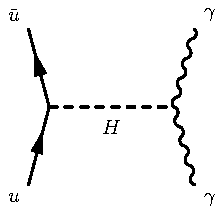
\includegraphics[width=0.2\textwidth]{./Figures/uu_to_Hgamgam.eps}
}
\end{center}
\caption{Examples of processes which are {\color{red} NOT} allowed in the Standard Model, with a quick explanation of why they are not allowed.}
\label{fig:forbidden_feyn}
\end{figure}



\section{Special relativity and units}

In particle physics it is customary to choose a system of units in which the value of the Planck constant $\hbar$ and the speed of light $c$ are both set to unity: $\hbar = c = 1$. Energy and momentum are therefore measured with the same units. Often the electronvolt (eV) is the energy unit chosen. For the applications of this experiment, we will be using MeV, GeV and TeV. Because of the Heisenberg uncertainty principle, the unit for space is also fixed: 

\begin{align}
\Delta p \Delta x \sim \hbar = 1 \implies [x] = \frac{1}{[p]}  = \frac{1}{\mathrm{MeV}}
\end{align}

Likewise, from $\Delta E \Delta t \sim \hbar = 1$, it follows that time has the same units of space. From $E=mc^2$, it follows that mass and energy have the same units. 


The particle free motion is described in terms of their energy $E$ and momentum $\mathbf{p}$. The three momentum components and the energy form a so-called 4-vector. You already have the knowledge of what a 4-vector is, but probably nobody has used this name just yet. Let's start from a standard position vector in space $\mathbf{x}$, with components $(x,y,z)$ in a given reference frame $S$. Let's name this a 3-vector (and you can probably already guess where I am going...). You know well that in special relatively the spacial coordinates and the time of a given event cannot be treated independently from each other, simply because they mix if one describes the same event from a different reference frame in uniform motion with respect to the original one.  For a change of reference frame from a frame $S$ to one $S'$ moving with speed $v$ along $\hat{x}$ with respect to $S$, the 4-vector transforms into $(\mathbf{x'},t')$ such that:

\begin{align}
x' &= \gamma \left(x + \beta t\right) \nonumber \\
y' &= y \nonumber \\
z' &= z \nonumber\\
t' &= \gamma \left(t + \beta x\right)
\end{align}
\label{eq:lorentz_transform}

\noindent where we are using units in which the speed of light $c$ is equal to 1. $x'$ is a function of both $x$ and $t$, and the same is true for $t'$.  Perfect! Let's then define a 4-vector as $x_\mu = (x,y,z,t)$. The components of a 4-vector transform by Lorentz boost as in Eq.~\ref{eq:lorentz_transform}.

The symbols $\gamma$ and $\beta$ are defined (for $c=1$) by: 

\begin{align}
\gamma = \frac{1}{\sqrt{1-v^2}} \qquad \beta = \frac{v}{c} = v
\end{align}

The transformations in Eq.~\ref{eq:lorentz_transform} are such that the product  

\begin{align}
s = t^2 - \mathbf{x} \cdot \mathbf{x}
\end{align}

\noindent is invariant for Lorentz transformations, that is, its value is the same in the reference frame $S$ or in any other boosted frame $S'$. 

\begin{exercise}
Prove it! Prove that  $t^2 - \mathbf{x} \cdot \mathbf{x} =  t'^2 - \mathbf{x'} \cdot \mathbf{x'}$, where the primed quantities are connected to the non-primed ones by a Lorentz transformation like in eq.~\ref{eq:lorentz_transform}
\end{exercise}

So, momentum and energy form another 4-vector, $p_{\mu} = (p_x,p_y,p_z,E)$. That means that if I go from one reference frame to another in relative motion along $\hat{x}$,

\begin{align}
p_x' &= \gamma \left(p_x + \beta E\right) \nonumber \\
p_y' &= p_y \nonumber \\
p_z' &= p_z \nonumber\\
E' &= \gamma \left(E + \beta p_x\right)
\end{align}
\label{eq:lorentz_transform_momentum}

It also means that $E^2 - \mathbf{p}\cdot \mathbf{p}$ is an invariant.......

\subsection{Invariant Mass}
\label{sec:invariant_mass}

The fact that for a 4-vector of type $\left(\mathbf{m}_x, m_t\right)$ the product $s_{m} = m_t^2 - \mathbf{m}_x \cdot \mathbf{m}_x$ is Lorentz-invariant (that is, it is the same in every reference frame, regardless of its boost) is general. The number $\sqrt{s_{m}} = \sqrt{m_t^2 - \mathbf{m}_x \cdot \mathbf{m}_x}$ is the \textit{magnitude} of the 4-vector. As pointed out earlier, the energy and momentum form a 4-vector $\left(\mathbf{p},E\right)$. Therefore the combination $s = E^2-p^2$ (where $p$ indicates the magnitude of $\mathbf{p}$) is Lorentz-invariant. What is the value of this Lorentz-invariant quantity? Let's consider a particle of mass $m$. In its own rest frame: 

\begin{align} 
E &= m \\ 
\mathbf{p} &= 0 \\ 
s^2 &= E^2 - p^2 = m^2
\end{align}

\noindent But since $s^2$ is Lorentz-invariant, \textit{this mathematical combination of the momentum and the energy of the particle will yield the particle mass regardless of the rest frame where it is computed!}. We will use this fact repeatedly.

\section{Proton-proton Collisions - Collider Physics Variables}
\label{sec:collider_physics_variables}

In this experience, we will study proton-proton collisions produced by the LHC and recorded by ATLAS. The LHC collides two beams of protons head-on. The energy of the protons in each beam is $\ebeam = 6.5\ \TeV$. 

As said earlier, protons are not elementary particles. They are made by three \textit{valence} quarks (two $u$ and one $d$) and a \textit{sea} of other quark-antiquark pairs and gluons, which are created and destroyed continuously according to quantum mechanics. All these particles (the valence quarks and the sea quarks and gluons) take the generic name of \textit{partons}. 

The scale for the proton binding energy is given by its own mass ($\sim 1\ \GeV$). With respect to the typical energy transfer in a LHC collision of interest, with energy exchanged of hundreds of GeV, the binding energy of the proton is small. Therefore the partons in the proton in a LHC collision \textbf{can be considered as free}: the LHC is indeed a parton collider. 

Partons inside a proton however do not have the same energy/momentum as the proton of course: it is the sum of the energies and momenta of all partons that will yield the energy and momentum of the proton. Let's say that each parton $i$ in the collision carries a fraction $x_i$ of the momentum and energy of the proton. The 4-vectors of the protons and colliding partons are (neglecting all masses, and setting the $\hat{z}$ as beam axis) 

\begin{align}
\mathrm{Proton 1}&: \left(0,0,\ebeam,\ebeam\right) \\
\mathrm{Proton 2}&: \left(0,0,-\ebeam,\ebeam\right) \\
\mathrm{Parton 1}&: \left(0,0,x_1\ebeam,x_1\ebeam\right) \\
\mathrm{Parton 2}&: \left(0,0,-x_2\ebeam,x_2\ebeam\right) \\
\end{align}

The magnitude of the 4-vector corresponding to the sum of the two proton 4-vectors is 

\begin{align}
\sqrt{s} = \sqrt{\left(2\ebeam\right)^2 - \left(\ebeam-\ebeam\right)^2} = \sqrt{4\ebeam^2} = 2\ebeam = 13\ \TeV
\end{align}

\noindent which is known as the centre-of-mass energy of the LHC. However, this is \textbf{not} the centre of mass energy of the parton-parton collisions! The actual particles colliding are the partons. Their own centre-of mass energy is:

\begin{align*}
\sqrt{\hat{s}} = \sqrt{\left( x_1 + x_2 \right) ^2 \ebeam^2 - \left( x_1 - x_2\right)^2 \ebeam^2}
\end{align*}

\begin{exercise}
Prove that this implies $\sqrt{\hat{s}} = \sqrt{x_1 x_2} \sqrt{s}$
\end{exercise}

By the way: the frame in which the proton-proton collision happens at rest (the laboratory frame) does not coincide with that in which the parton collision happens at rest. With respect to the laboratory frame, the parton-parton collision happens in a system which is boosted along the beam axis by $p_{\mathrm{boost}} = |x_1-x_2| \ebeam$.

 \begin{figure}[!h]
\begin{center}
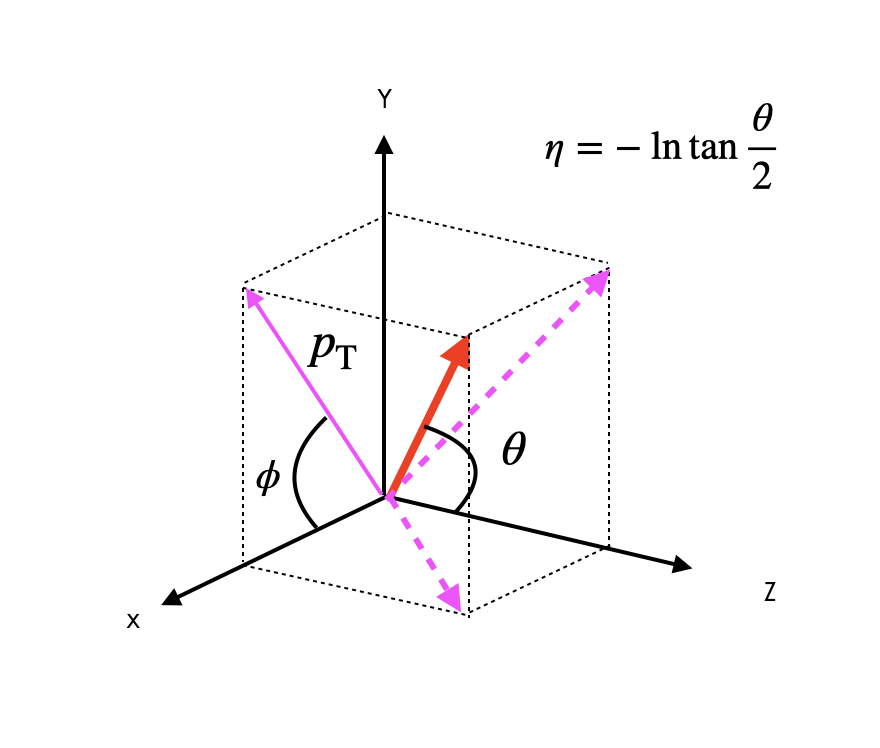
\includegraphics[width=0.5\textwidth]{./Figures/collider_physics_variables.png}
\end{center}
\caption{Diagram of the kinematic variables used at a hadron collider. The $z$ axis coincides with the beam axis.}
\label{fig:collider_variables}
\end{figure}


Let's recap: on an \textbf{event-by-event basis}, the parton-parton collision happens in a frame with a different boost with respect to the laboratory frame, and the collision energy is smaller than the nominal proton-proton centre-of-mass energy. 

\begin{exercise}
The mass of the top quark is 172 GeV. The SppS, a collider colliding protons and antiprotons at CERN, worked up to energies of $\sqrt{s} = 900\ \GeV$. Yet, we had to wait for the Tevatron ($\sqrt{s} = 1.8\ \TeV$) for the top quark discovery. Why?
\end{exercise}

\begin{exercise}
Draw one of the most relevant Feynman diagram for the production of the following particles at the LHC. If quarks are involved, specify if they are likely to be valence or sea quarks: $Z$ boson production, $W$ boson production, $t\bar{t}$ production.
\end{exercise}

\begin{exercise}
The mass of the $W$ boson is $m = 80\ \GeV$. In a given collision pp collision at $\sqrt{s} = 13\ \TeV$, the $W$ boson is produced by a collision of a valence quark with $x = 0.3$,  and a sea quark. Find $x$ of the sea quark and compute $p_{\mathrm{boost}}$ for this collision.
\end{exercise}


So, in practice what happens is that in each event, the LHC experiments look at a collision happening with an unknown boost along the $\hat{z}$ axis. There is one important implication: if we measure any variable which is not Lorentz-invariant, we would make a big confusion when measuring it in many events, because we would mix up values belonging to different reference frames! This implies we have to carefully choose the quantities that we measure at a hadron collider like the LHC to characterise the particles' final states: we should avoid using any variable relying on \textit{longitudinal} quantities, that is, quantities relying on variables measured along the $\hat{z}$ axis. The reason  Therefore, the variables we use at a hadron collider are (see also Figure~\ref{fig:collider_variables}) 

\begin{itemize}
\item The momentum in a plane transverse to the beam, $\pt$.
\item The angle $\phi$ in the transverse plane with respect to the direction pointing towards the LHC centre.
\item The mass.
\end{itemize}

And now we have a problem, because three variables do not determine a 4-vector, of course. We need somewhat to provide the direction with respect to the beam axis. This is done with the rapidity $y$ variable, or with its approximated variable (valid for massless particles) the pseudorapidity $\eta$. 

\begin{align*}
y &= \frac{1}{2} \ln \left(\frac{\mathbf{E} + p_z}{\mathbf{E} + p_z} \right) \\
\eta &= -\ln \tan \frac{\theta}{2}
\end{align*}

\section{Cross-section and luminosity}
\label{sec:cross_section_lumi}

Imagine you have a beam of particles impinging on a slab of targets, and that the targets are small enough that you can neglect shielding effects of one target with respect to another. The total number of interactions that you will observe per unit time will be determined by:

\begin{itemize}
\item characteristics of the beam of particles (how many particles per unit surface per unit time you are shooting, that is, the incoming flux of particles),
\item the target density,
\item the transverse area that the targets offer to the beam, that is, the cross-section of the individual targets. 
\end{itemize}

Inheriting this language, we define the cross-section and the luminosity of a given process at a hadron collider such that the number of occurrences of that process that we observe per unit time is given by: 

\begin{align}
\frac{dN}{dt} = \sigma \times \mathcal{L}
\end{align} 

In the example above, the luminosity is something connected with how many protons per beam we have, how many beams are circling the LHC, etc., while the cross-section is intrinsically connected with the physical interaction yielding a given process. The cross-section units are those of a surface (cm$^2$, for example\footnote{Particle physics cross sections are normally expressed in barns, where $1\ \mathrm{barn} = 10^{-24}\ \mathrm{cm}^2$}), while those of the luminosity are

\begin{align}
[\mathcal{L}] =  [\mathrm{surface}]^{-1}\cdot [\mathrm{time}]^{-1}.
\end{align}

A typical number $\mathcal{L}$ during the LHC Run 2 is $\mathcal{L} \sim 2\times 10^{34}$ cm$^{-2}$ s$^{-1}$. The total number of events we will count for a given process in a given period of time is of course given by 

\begin{align}
N = \int_{\Delta T} \frac{dN}{dt} dt = \int_{\Delta T} \sigma \times \mathcal{L} dt &= \sigma \int_{\Delta T} \mathcal{L} dt = \sigma \Lint, \\ 
\Lint &= \int_{\Delta T} \mathcal{L} dt.
\end{align}

The data collected by a given experiment over a period of time are typically expressed with the corresponding \textit{integrated luminosity} $\Lint$. Let's make an example. The ATLAS experiment has collected a number of proton-proton collisions corresponding to $\Lint = 139\ \ifb$ during the so-called Run 2 at $\sqrt{s} = 13\ \TeV$. The production cross-section for top pairs is predicted to be $\sigma_{t\bar{t}} = 831\ \mathrm{pb}$. Let's compute how many top pair production events we expect to have collected during the full Run 2: 

\begin{align}
N_{t\bar{t}} = \sigma_{t\bar{t}} \times \Lint &= 831 \times 10^{-12} \ \mathrm{barns} \times 139 \times \left(10^{-15}\ \mathrm{barns}\right)^{-1} \\
N_{t\bar{t}} &= 1.16\times 10^{8}
\end{align}

So, we expect something like 116 million top pairs to have been produced during Run 2 in ATLAS. 

\begin{figure}[tb] 
	\begin{center}
	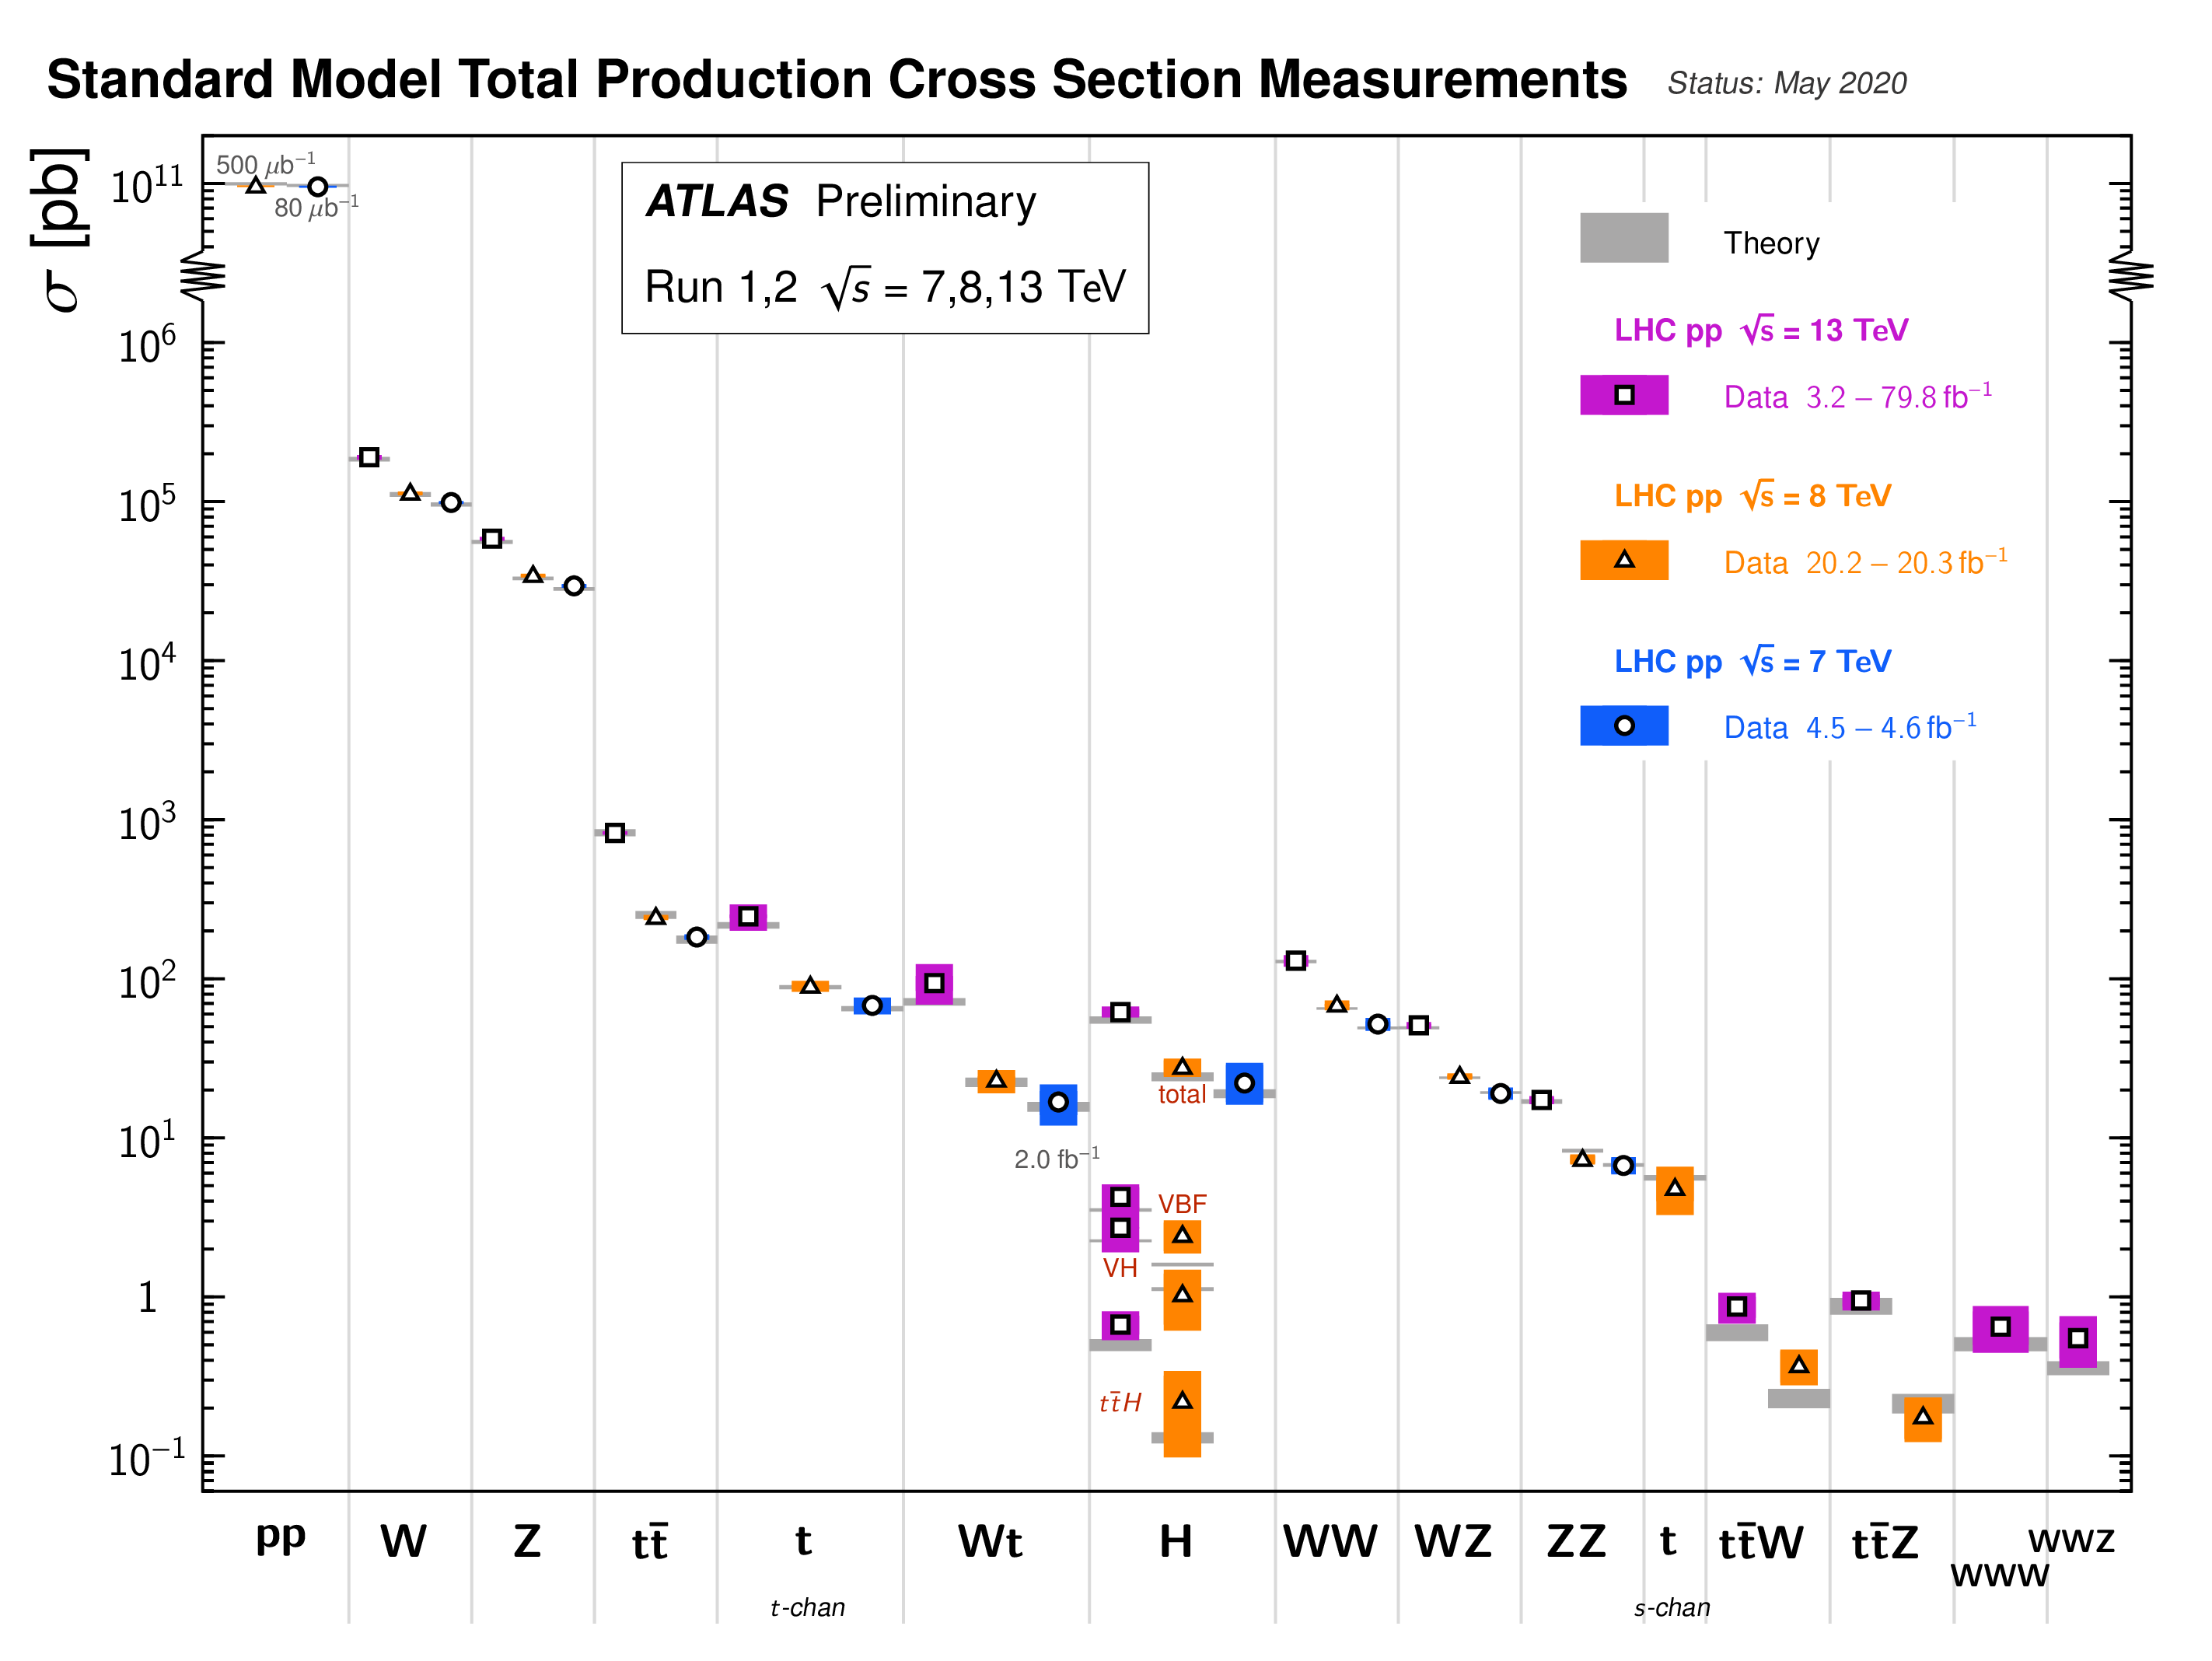
\includegraphics[width=0.7\columnwidth]{Figures/SM_summary.png}
	\end{center}
	\caption{Predictions and ATLAS measurements for the production cross sections of several Standard Model processes. Taken from Ref.~\cite{SM_summary}.}
	\label{fig:SM_summary_plot}
\end{figure}

Now, let's take a close look at Figure~\ref{fig:SM_summary_plot}. It shows the cross-sections for several SM processes at the LHC, for different proton-proton centre-of-mass energies. The proton-proton inelastic cross-section at $\sqrt{s} = 13\ \TeV$ is about $80$ mb. Let's consider one random process as an example, say $WW$ production. The plot tells us that the production cross section is between 100 and 200 pb - let's take 160 pb. So, from the ratio of these numbers, we learn that only one in 500,000 proton-proton collisions will produce $WW$. 

\begin{exercise}
From Figure~\ref{fig:SM_summary_plot}, the Higgs boson production cross-section is $\sigma = 80$ pb. Compute how many Higgs bosons LHC has produced during Run 2, and using the typical value for $\mathcal{L}$ given above, compute how many Higgs bosons per minute the LHC is producing when running at that luminosity. 
\end{exercise}
